\documentclass{standalone}
\usepackage{tikz}
\usetikzlibrary{automata,positioning}

\begin{document}
  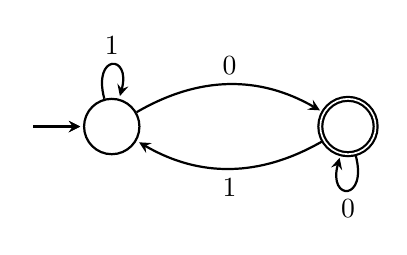
\begin{tikzpicture}[%
    >=stealth,
    shorten >=1pt,
    node distance=3cm,
    on grid,
    auto,
    state/.append style={minimum size=2em},
    thick
  ]
    \node[state, initial, initial text = {}] (A) {};
    \node[state, accepting] (B) [right of=A] {};

    \path[->] (A) +(-1,0) edge (A)
              (A)         edge [loop above] node {$1$} (A)
              (A)         edge [bend left]  node {$0$} (B)
              (B)         edge [loop below] node {$0$} (B)
              (B)         edge [bend left]  node {$1$} (A);
  \end{tikzpicture}
\end{document}